\subsection{Navegación en Google Maps}
        La API está compuesta por una interfaz compuesta principalmente por el mapa,         por el cual se puede navegar por todo el mapa del mundo. Para desplazarse,          hay que realizar alguna de las siguientes acciones:
     \begin{itemize} 
        \item Arrastrar el mapa.
        \item Pulsar alguna de las teclas direccionales.
        \item Usar de los controles de navegación.
     \end{itemize} 
     
      \hspace*{1cm}Los controles de navegación de Google Maps se muestran a la izquierda del mapa por lo general.
En la figura \ref {fig:Cap2_3_1} se podra ver un ejemplo de los controles, cabe mencionar que algunas páginas web que usan la API pueden no ofrecer los mismos controles de navegación. Ya que se pueden configurar para no aparecer:\\
    \begin{enumerate}
      \item Flechas para mover manualmente el mapa, el boton del centro te devuelve             a la vista original.
      \item Boton para hacer un acercamiento de manera manualmente.
      \item Una barra que tambien permite realizar un acercamiento al mapa.
     \end{enumerate} 
     
    \begin{figure}[hbtp]
        \centering
            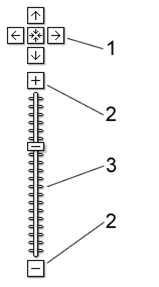
\includegraphics{Imagenes/Cap2_3_1.png}
            \caption{Los botones de la API}
            \label{fig:Cap2_3_1}
    \end{figure}
    
     \subsubsection{Tipos de vistas}
        Existen distintas vistas disponibles en Google Maps. En la esquina superior          derecha del mapa se pueden observar algunos de los modos:
    \begin{itemize} 
         \item Mapa: muestra un mapa con una presentación tradicional de carreteras             ,parques, fronteras, cuerpos de agua, etc.
          \item Satélite: muestra imágenes aéreas. Para ver los nombres de las                 calles y otro tipo de información, activa Superponer callejero.
          \item Terreno: muestra las elevaciones físicas en forma de relieves                      sombreados. También incluye los nombres de las calles e información                 adicional.
     \end{itemize} 
    
    En la figura \ref {fig:Cap2_3_2} se puede ver los distintos tipos de vistas
     
    \begin{figure}[hbtp]
        \centering 
            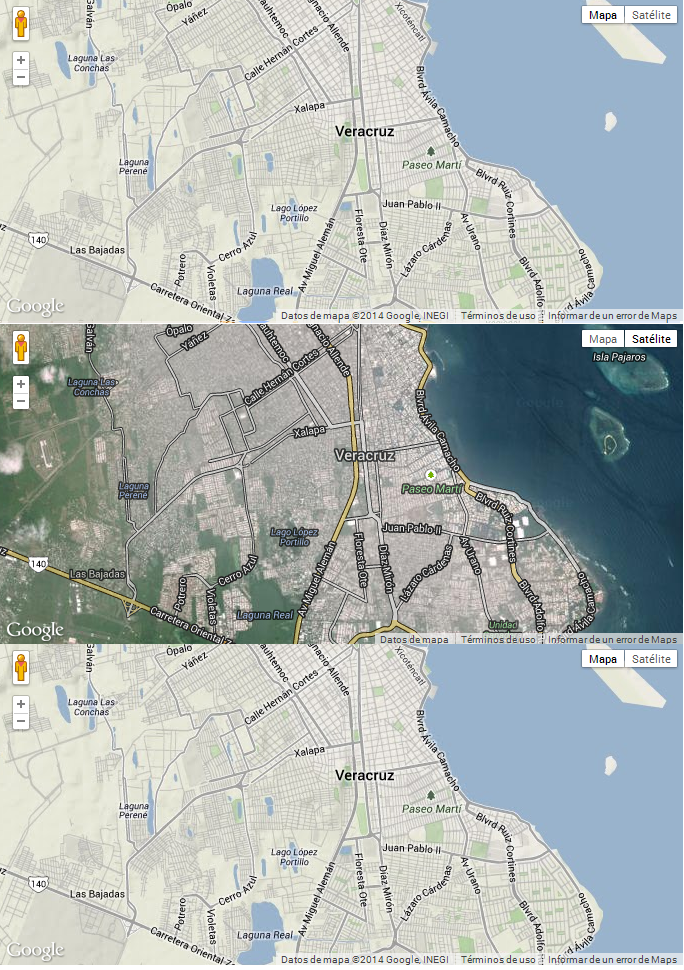
\includegraphics[width=0.5\textwidth]{Imagenes/Cap2_3_2.png}
            \caption{Vista de mapa, satelite y terreno respectivamente}  
            \label{fig:Cap2_3_2}
    \end{figure}
    
    
    \subsubsection{Como incluirlo en una pÁgina HTML}
    Primero se necesita introducir un codigo en un archivo .html:
\begin{lstlisting}[language=HTML, caption=Ejemplo simple, label=lst:codigo1]
<!DOCTYPE html>
<html>
    <head>
        <meta name="viewport" content="initial-scale=1.0, user-scalable=no" />
        <!-- Aqui va la hoja de estilos-->
        <style type="text/css">
            html { height: 100% }
            body { height: 100%; margin: 0; padding: 0 }
            #map_canvas { height: 50% }
        </style>
        <!-- Aqui se encuentra la API de Google maps-->
        <script type="text/javascript" src="http://maps.googleapis.com/maps/api/js?sensor=true"></script>
            <!-- El siguiente script incluye el metodo para inicializar la API, con la configuracion mencionada y referencia la etiqueta del cuerpo-->
            <script type="text/javascript">
            function initialize() {
            var mapOptions = {
            center: new google.maps.LatLng(-34.397, 150.644),
            zoom: 8,
            mapTypeId: google.maps.MapTypeId.ROADMAP
            };
            var map = new google.maps.Map(document.getElementById("map_canvas"),mapOptions);
            }
        </script>
    </head>
    <!-- El cuerpo  del metodo , aqui se agrega la etiqueta que contendra la API-->
        <body onload="initialize()">
        <div id="map_canvas" style="width:50%; height:50%"></div>
    </body>
</html>

\end{lstlisting}
El codigo \ref{lst:codigo1} es un ejemplo simple, esto es lo que se observa al compilar y visualizar:\\

    \begin{figure}[hbtp]
        \centering
            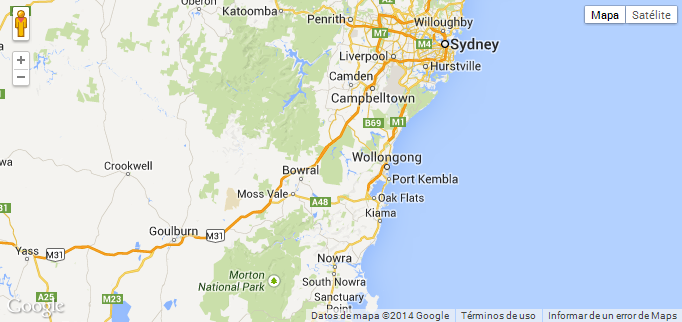
\includegraphics{Imagenes/Cap2_3_3.png}
            \caption{Vista del mapa de acuerdo al código puesto} 
            \label{fig:Cap2_3_3}
    \end{figure}
    
 \hspace*{1cm}De acuerdo a la figura \ref {fig:Cap2_3_3} muestra el mapa mostrando Sidney, Australia; de acuerdo a la configuración en el método de initialize().
 
\subsubsection{Creando un marcador}
Para crear un marcador, hay que valerse del objeto marker. Este objeto recibe un único argumento de opciones. Este argumento es un objeto literal que puede tener varias propiedades de las cuales tan solo dos son obligatorias:\\

\begin{itemize}
    \item Map.- Map es una referencia al mapa al que se quiera añadir el mapa. Es la variable que almacenamos cuando creamos el mapa.
    \item Position.- Esta propiedad establece la posición del marcador y es del tipo google.maps.LatLng.
\end{itemize}


Conociendo esto hay que declarar la siguiente linea de codigo como se puede ver en el codigo \ref{lst:codigo2} dentro del metodo initialize() del codigo anterior (codigo \ref{lst:codigo1}), en la figura \ref {fig:Cap2_3_4} se podra ver de forma grafica:\\

\begin{lstlisting}[language=HTML, caption=Marcador, label=lst:codigo2]
var marcador= new google.maps.Marker({
    position: new google.maps.LatLng(-34.397, 150.644),
    map: map
})
\end{lstlisting}

    \begin{figure}[hbtp]
        \centering
            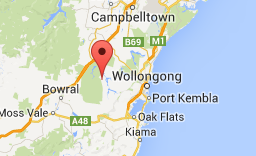
\includegraphics[width=0.3\textwidth]{Imagenes/Cap2_3_4.png}
            \caption{Marcador}  
            \label{fig:Cap2_3_4}
    \end{figure}
    

\hspace*{1cm}En la mayoría de las ocasiones, se necesitara añadir una descripcion emergente (Tooltip) al marcador de manera que cuando un usuario pase el ratón sobre el marcador, aparezca algo de información sobre este. Hacerlo es tan fácil como añadir una propiedad title al objeto de opciones del marcador (codigo \ref{lst:codigo3}), en la figura la figura \ref {fig:Cap2_3_5} se podra ver graficamente.\\

\begin{lstlisting}[language=HTML, caption=Descripción emergente, label=lst:codigo3]
    title: '¿Que lugar es este'
\end{lstlisting}

    \begin{figure}[hbtp]
        \centering
            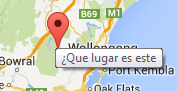
\includegraphics[width=0.3\textwidth]{Imagenes/Cap2_3_5.png}
            \caption{Marcador con descripción}    
            \label{fig:Cap2_3_5}
    \end{figure}

\hspace*{1cm}Tambien se puede cambiar el icono del marcador, al momento de crear un marcador (y en cualquier momento) podemos especificar una URL (absoluta o relativa) en la propiedad icon del objeto de propiedades del marcador, en el codigo \ref{lst:codigo4} y en la figura \ref {fig:Cap2_3_6} se podra ver.\\

\begin{lstlisting}[language=HTML, caption=Ícono de marcador, label=lst:codigo4]
    icon: 'http://google-maps-icons.googlecode.com/files/administration.png'
\end{lstlisting}

    \begin{figure}[hbtp]
        \centering
            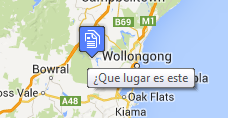
\includegraphics[width=0.3\textwidth]{Imagenes/Cap2_3_6.png}
            \caption{Marcador con otro icono}      
            \label{fig:Cap2_3_6}
    \end{figure}    

\subsubsection{Lineas y Polilineas}
   Para trazar líneas o poli-líneas con los mapas tenemos que utilizar la clase
   “google.maps.Polyline”, que nos proporciona Google Maps en su API, las propiedad    es que vamos a utilizar son las siguientes:\\
   
    \begin{itemize} 
         \item clickableboolean: Indica si este objeto controla eventos click. Por                 defecto el valor es true.
         \item map: Es el mapa en el que se va a mostrar la poli línea.
         \item path: Es la secuencia ordenada de coordenadas de la poli línea. 
         \item strokeColorstring: Contiene el color. En este ejemplo utilizamos este                : “#222000”, aunque puedes poner cualquier color CSS3 salvo los                     nombres de colores. 
         \item strokeOpacitynumber: Muestra la opacidad del trazo, es decir,                       determina lo transparente que será la línea, los valores estarán                    entre 0,0 y 1,0. 
         \item strokeWeightnumber: Muestra la anchura del trazo. 
    \end{itemize} 
    
     \hspace*{1cm}El código que hemos utilizado es igual que el de los ejemplos anteriores,           solamente hemos añadido la poli línea que hemos dibujado a través del objeto        “google.maps.Polyline”.\\
    Primero se dibuja la ruta, creamos el array ruta en el que ponemos los siguiente     s valores, quedaria como el codigo \ref{lst:codigo5}:\\
    
    \begin{lstlisting}[language=HTML, caption=Array de rutas, label=lst:codigo5]
    	var ruta =[
    		new google.maps.LatLng(-34.397, 150.644),
    		new google.maps.LatLng(-33.7, 149.09),
    		new google.maps.LatLng(-34.2, 150.666),
    	];
    \end{lstlisting}
    
     \hspace*{1cm}Después creamos el objeto “líneas” al que le vamos a pasar los puntos que queremos que dibuje a través del array ruta (como se puede ver en en el codigo \ref{lst:codigo6}, este es el código, en la figura \ref {fig:Cap2_3_7} se podra ver graficamente:\\
    
    \begin{lstlisting}[language=HTML, caption=Polilinea, label=lst:codigo6]
    	var lineas= new google.maps.Polyline({
				path: ruta,
				map: map,
				strikeColor: '#900',
				strokeWeight: 10,
				strokeOpacity: 1,
				clickable: false
			});
    \end{lstlisting}
    
    \begin{figure}[hbtp]
        \centering
            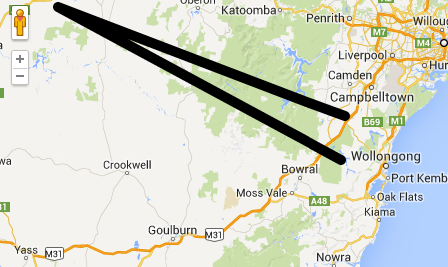
\includegraphics{Imagenes/Cap2_3_7.png}
            \caption{Ruta hecha con polilineas}   
            \label{fig:Cap2_3_7}
    \end{figure}   
    
    \subsubsection{Rutas}
    Ahora vamos a ver cómo cargar una ruta con Google Maps v3.
Ahora vamos a definir la Ruta. Para la Ruta tenemos que saber que Google Maps nos ofrece un par de objetos. El primero y más importante es google.maps.DirectionsService. Este objeto será el encargado de calcularnos una ruta y devolvernos un objeto DirectionsResult con toda la información de la ruta.
Para que el objeto DirectionsService nos calcule la ruta le tenemos que pasar un objeto DirectionsRequest indicándole la información de la ruta: origen, destino, forma de desplazamiento,etc por ahora solo nos ocuparemos de estas 3, en el código \ref{lst:codigo7}.\\

    \begin{lstlisting}
    [language=HTML, caption=Coordenadas de origen-destino, label=lst:codigo7]
        <!--Coordenadas, origen, destino y camino, en este caso es en automovil-->
    	var request={
    		origin :"(-34.397, 150.644)",
    		destination : "(-33.4, 149.644)",
    		travelMode: google.maps.TravelMode.DRIVING
    	};
    \end{lstlisting}
    
\hspace*{1cm}Este objeto DirectionsRequest se lo pasamos al DirectionsService para que calcule la ruta. Para ello ejecutamos el método .route() como se puede ver en en el código \ref{lst:codigo8}.\\

    \begin{lstlisting}[language=HTML, caption=Cálculo de la ruta, label=lst:codigo8]
        <!--Calcula una ruta usando la variable "request" como parametro-->
        var ser = new google.maps.DirectionsService();
        ser.route(
        	request,function(res,sts) {
        		if(sts=='OK')ren.setDirections(res);	
        	}
        );	
    \end{lstlisting}

\hspace*{1cm}El resultado del método .route() devuelve el DirectionsResult dentro del atributo result.
Una vez que tenemos el Resultado podemos hacer dos cosas. La primera será explotarlo para acceder a toda la información que contiene de las rutas y la segunda será representarlo visualmente. Para este segundo caso contamos con el objeto google.maps.DirectionsRenderer. Dicho objeto es capaz de renderizar un mapa o un texto con un DirectionsResult como se puede ver en en el codigo \ref{lst:codigo9} .\\
Para configurar el DirectionsRender utilizamos .setMap() para indicarle cual es el mapa -objeto Map- y .setPanel() para saber cual es la capa del documento HTML en la que volcar la ruta.\\

    \begin{lstlisting}[language=HTML, caption=Etiqueta que graficará el camino, label=lst:codigo9]
        <!--El objeto DirectionsRender se pondra en una etiqueta, en este caso "directionsPanel"-->
        var ren = new google.maps.DirectionsRenderer( {'draggable':true} );
        ren.setMap(map);
        ren.setPanel(document.getElementById("directionsPanel"));
    \end{lstlisting}
      
En la figura \ref {fig:Cap2_3_8} es lo que se vera en pantalla:

    \begin{figure}[hbtp]
        \centering
            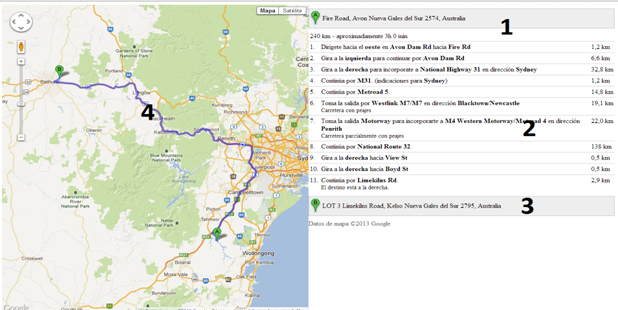
\includegraphics{Imagenes/Cap2_3_8.png}
            \caption{Ruta usando los objetos DirectionResult y DirectionRenderer}                       \label{fig:Cap2_3_8}
    \end{figure}   

\hspace*{1cm}En la figura \ref {fig:Cap2_3_8}  podemos observar los siguientes puntos:\\
 \begin{enumerate}
    \item Punto de Partida
    \item Caminos que debe de tomar para llegar al destino o punto 3
    \item Punto de destino
    \item Mapa que muestra gráficamente el punto 2
 \end{enumerate}


